% The acoustic model configurations (Ch. 4).
\documentclass[12pt,border=2pt]{standalone}
\usepackage[T1]{fontenc}\usepackage{newtxtext}
\usepackage{tikz}\usetikzlibrary{positioning,arrows.meta,calc}
\begin{document}
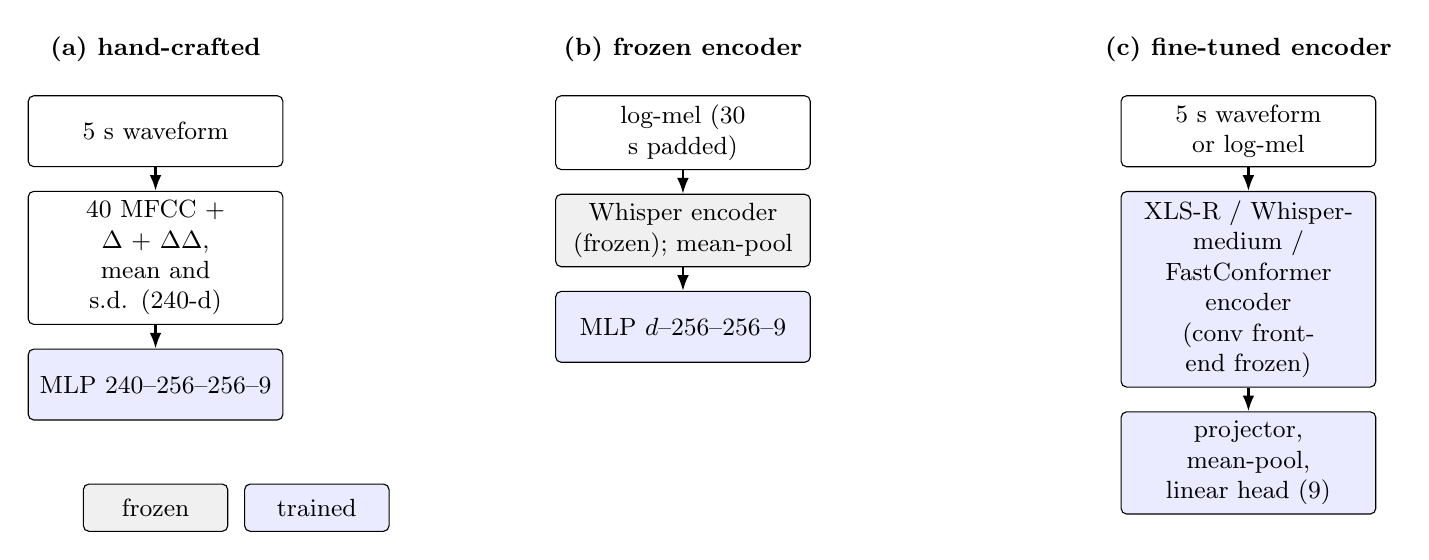
\begin{tikzpicture}[node distance=3mm and 5mm,
  box/.style={draw, rounded corners=2pt, align=center, font=\small, minimum height=9mm, text width=30mm, fill=white},
  frozen/.style={box, fill=black!6}, train/.style={box, fill=blue!8},
  arr/.style={-{Latex[length=2mm]}, thick}]
  \node[font=\small\bfseries] (t1) {(a) hand-crafted};
  \node[box, below=of t1] (a1) {5 s waveform};
  \node[box, below=of a1] (a2) {40 MFCC + $\Delta$ + $\Delta\Delta$,\\mean and s.d. (240-d)};
  \node[train, below=of a2] (a3) {MLP 240--256--256--9};
  \draw[arr] (a1) -- (a2); \draw[arr] (a2) -- (a3);
  \node[font=\small\bfseries, right=36mm of t1] (t2) {(b) frozen encoder};
  \node[box, below=of t2] (b1) {log-mel (30 s padded)};
  \node[frozen, below=of b1] (b2) {Whisper encoder\\(frozen); mean-pool};
  \node[train, below=of b2] (b3) {MLP $d$--256--256--9};
  \draw[arr] (b1) -- (b2); \draw[arr] (b2) -- (b3);
  \node[font=\small\bfseries, right=36mm of t2] (t3) {(c) fine-tuned encoder};
  \node[box, below=of t3] (c1) {5 s waveform or log-mel};
  \node[train, below=of c1] (c2) {XLS-R / Whisper-medium /\\FastConformer encoder\\(conv front-end frozen)};
  \node[train, below=of c2] (c3) {projector, mean-pool,\\linear head (9)};
  \draw[arr] (c1) -- (c2); \draw[arr] (c2) -- (c3);
  \node[frozen, below=8mm of a3, text width=16mm, minimum height=6mm] (l1) {frozen};
  \node[train, right=2mm of l1, text width=16mm, minimum height=6mm] (l2) {trained};
\end{tikzpicture}
\end{document}
